 \documentclass[UTF8,a4paper,12pt]{ctexbook} 
 
 \usepackage{graphicx}%学习插入图
 \usepackage{verbatim}%学习注释多行
 \usepackage{booktabs}%表格
 \usepackage{geometry}%图片
 \usepackage{amsmath}
 \usepackage{amssymb}
 \usepackage{listings}%代码
 \usepackage{xcolor}  %颜色
 \usepackage{enumitem}%列表格式
 \usepackage{tcolorbox}
 \usepackage{algorithm}  %format of the algorithm
 \usepackage{algorithmic}%format of the algorithm
 \usepackage{multirow}   %multirow for format of table
 \usepackage{tabularx} 	%表格排版格式控制
 \usepackage{array}	%表格排版格式控制
 \usepackage{hyperref}
 \CTEXsetup[format+={\flushleft}]{section}
 
 \newcommand{\EQ}[1]{$\textbf{EQ:}#1\ $}
 \newcommand{\ALGORITHM}[1]{$\textbf{Algorithm:}#1\ $}
 \newcommand{\Figure}[1]{$\textbf{Figure }#1\ $}
 
 \renewcommand{\figurename}{Fig}
 \geometry{left=1.6cm,right=1.8cm,top=2cm,bottom=1.7cm} %设置文章宽度
 
 \pagestyle{plain} 		  %设置页面布局
 \author{\kaishu 郑华}
 \title{\heiti 算法解题笔记}
  %代码效果定义
  \definecolor{mygreen}{rgb}{0,0.6,0}
  \definecolor{mygray}{rgb}{0.5,0.5,0.5}
  \definecolor{mymauve}{rgb}{0.58,0,0.82}
  \lstset{ %
  	backgroundcolor=\color{white},   % choose the background color
  	basicstyle=\footnotesize\ttfamily,        % size of fonts used for the code
  	%stringstyle=\color{codepurple},
  	%basicstyle=\footnotesize,
  	%breakatwhitespace=false,         
  	%breaklines=true,                 
  	%captionpos=b,                    
  	%keepspaces=true,                 
  	%numbers=left,                    
  	%numbersep=5pt,                  
  	%showspaces=false,                
  	%showstringspaces=false,
  	%showtabs=false,        
  	columns=fullflexible,
  	breaklines=true,                 % automatic line breaking only at whitespace
  	captionpos=b,                    % sets the caption-position to bottom
  	tabsize=4,
  	commentstyle=\color{mygreen},    % comment style
  	escapeinside={\%*}{*)},          % if you want to add LaTeX within your code
  	keywordstyle=\color{blue},       % keyword style
  	stringstyle=\color{mymauve}\ttfamily,     % string literal style
  	frame=single,					%tb top and bottom; L left double line
  	xleftmargin=.06\textwidth, 
  	%xrightmargin=.1\textwidth,
  	rulesepcolor=\color{red!20!green!20!blue!20},
  	% identifierstyle=\color{red},
  	language=c++,
  }
 
 \begin{document}          %正文排版开始
 	\maketitle
 	\tableofcontents
 	
\chapter{算法基础}
	\section{时间复杂度}
		\begin{table}[h]
			\centering
			\begin{tabular}{|p{2cm}<{\centering}|p{2cm}<{\centering}|p{2cm}<{\centering}|p{2cm}<{\centering}|p{2cm}<{\centering}|p{2cm}<{\centering}|p{2cm}<{\centering}|}	
				\hline
				n & $log_2^n$ & n$\times log_2^n$ & $n^2$ & $n^3$ & $2^n$ & $n!$ \\
				
				\hline
				4 & 2 		  & 8 				  & 16 	  & 64 	  & 16 	  &24 \\
				
				\hline
				8 & 3 		  & 24 				  & 64 	  & 512	  & 256 	  &80320 \\
				
				\hline
				10 & 3.32 	  & 33.2			 & 100 	  & 1000	  & 1024 	  &3628800 \\
				
				\hline
				16 & 4 		  & 64 				  & 256	  & 4096 	  & 65536	  &$2.1*10^{13}$ \\
				
				\hline
				32 & 5 		  & 160 			 & 1024   & 32768 	  & 4.3$\times 10^9$ 	  &$2.6*10^{35}$\\
				
				\hline
				128 & 7 	  & 896 			& 16384   & 2097152 	  & 3.4$\times 10^{38}$ 	  &$\infty$ \\
				
				\hline
				1024 & 10 	  & 10240 			& 1048576 & 1.07$\times 10^9$ 	  & $\infty$ 	  &$\infty$ \\
				
				\hline
				10000 & 13.29 & 132877 			& $10^8$  & $10^{12}$	  & $\infty$ 	  &$\infty$ \\
				\hline
			\end{tabular}
			\caption{各个函数随n的增长函数值的变化}
		\end{table} 
	
	\section{解题提醒}
		\subsection{等价意思..简化题目}
		
		\subsection{有无最优子结构} 即是否可以用数学公式简化模型。
		
		\subsection{想通可行再实践}
			
	\section{分治思想}
		\subsection{基本概念}
			在计算机科学中,分治法是一种很重要的算法。字面上的解释是“分而治之”,就是把一个复杂的问题分成两个或更多的相同或相似的子问题,再把子问题分成更小的子问题……直到最后子问题可以简单的直接求解,原问题的解即子问题的解的合并。这个技巧是很多高效算法的基础,如排序算法(快速排序,归并排序),傅立叶变换(快速傅立叶变换)……
		
			任何一个可以用计算机求解的问题所需的计算时间都与其规模有关。问题的规模越小,越容易直接求解,解题所需的计算时间也越少。例如,对于n个元素的排序问题,当n=1时,不需任何计算。n=2时,只要作一次比较即可排好序。n=3时只要作3次比较即可,…。而当n较大时,问题就不那么容易处理了。要想直接解决一个规模较大的问题,有时是相当困难的。
		
		\subsection{基本思想及策略}
			分治法的设计思想是:将一个难以直接解决的大问题,分割成一些规模较小的相同问题,以便各个击破,分而治之。
			
			分治策略是:对于一个规模为n的问题,若该问题可以容易地解决(比如说规模n较小)则直接解决,否则将其分解为k个规模较小的子问题,这些子问题互相独立且与原问题形式相同,递归地解这些子问题,然后将各子问题的解合并得到原问题的解。这种算法设计策略叫做分治法。
			
			如果原问题可分割成k个子问题,1<k≤n,且这些子问题都可解并可利用这些子问题的解求出原问题的解,那么这种分治法就是可行的。由分治法产生的子问题往往是原问题的较小模式,这就为使用递归技术提供了方便。在这种情况下,反复应用分治手段,可以使子问题与原问题类型一致而其规模却不断缩小,最终使子问题缩小到很容易直接求出其解。这自然导致递归过程的产生。分治与递归像一对孪生兄弟,经常同时应用在算法设计之中,并由此产生许多高效算法。
		
		\subsection{分治法适用的情况}
			分治法所能解决的问题一般具有以下几个特征:
			\begin{itemize}
				\item 该问题的规模缩小到一定的程度就可以容易地解决:绝大多数问题都可以满足的,因为问题的计算复杂性一般是随着问题规模的增加而增加;
				\item 该问题可以分解为若干个规模较小的相同问题,即该问题具有最优子结构性质:应用分治法的前提它也是大多数问题可以满足的,此特征反映了递归思想的应用;
				\item 利用该问题分解出的子问题的解可以合并为该问题的解:是关键,能否利用分治法完全取决于问题是否具有第三条特征,如果具备了第一条和第二条特征,而不具备第三条特征,则可以考虑用贪心法或动态规划法。
				\item 该问题所分解出的各个子问题是相互独立的,即子问题之间不包含公共的子子问题:涉及到分治法的效率,如果各子问题是不独立的则分治法要做许多不必要的工作,重复地解公共的子问题,此时虽然可用分治法,但一般用动态规划法较好
			\end{itemize}
		\subsection{基本步骤}
			分治法在每一层递归上都有三个步骤:
			
			\textbf{step1 分解}:将原问题分解为若干个规模较小,相互独立,与原问题形式相同的子问题;
			
			\textbf{step2 解决}:若子问题规模较小而容易被解决则直接解,否则递归地解各个子问题
			
			\textbf{step3 合并}:将各个子问题的解合并为原问题的解。
			
		\subsection{可使用分治法求解的一些经典问题}
			\begin{itemize}
				\item 二分搜索
				\item 大整数乘法
				\item Strassen矩阵乘法
				\item 棋盘覆盖
				\item 合并排序
				\item 快速排序
				\item 线性时间选择
				\item 最接近点对问题
				\item 循环赛日程表
				\item 汉诺塔
			\end{itemize}
		\subsection{依据分治法设计程序时的思维过程}
			1、一定是先找到最小问题规模时的求解方法
			
			2、然后考虑随着问题规模增大时的求解方法
			
			3、找到求解的递归函数式后(各种规模或因子),设计递归程序即可。
	\section{动态规划思想}
		\url{http://mp.weixin.qq.com/s/3h9iqU4rdH3EIy5m6AzXsg}
		
		\subsection{基本概念}
			动态规划过程是:每次决策依赖于当前状态,又随即引起状态的转移。一个决策序列就是在变化的状态中产生出来的,所以,这种多阶段最优化决策解决问题的过程就称为动态规划。
			
		\subsection{基本思想和策略}
			基本思想与分治法类似,也是将待求解的问题分解为若干个子问题(阶段),按顺序求解子阶段,前一子问题的解,为后一子问题的求解提供了有用的信息。在求解任一子问题时,列出各种可能的局部解,通过决策保留那些有可能达到最优的局部解,丢弃其他局部解。依次解决各子问题,最后一个子问题就是初始问题的解。
			
			由于动态规划解决的问题多数有重叠子问题这个特点,为减少重复计算,对每一个子问题只解一次,将其不同阶段的不同状态保存在一个二维数组中。
			
			与分治法最大的差别是:适合于用动态规划法求解的问题,经分解后得到的子问题往往不是互相独立的(即下一个子阶段的求解是建立在上一个子阶段的解的基础上,进行进一步的求解)。
		\subsection{适用的情况}
			能采用动态规划求解的问题的一般要具有3个性质:
			
			\textbf{(1) 最优化原理}:如果问题的最优解所包含的子问题的解也是最优的,就称该问题具有最优子结构,即满足最优化原理。
			
			\textbf{(2) 无后效性}:即\textbf{某阶段状态一旦确定,就不受这个状态以后决策的影响}。也就是说,某状态以后的过程不会影响以前的状态,只与当前状态有关。
			
			\textbf{(3) 有重叠子问题}:即子问题之间是不独立的,一个子问题在下一阶段决策中可能被多次使用到。(该性质并不是动态规划适用的必要条件,但是如果没有这条性质,动态规划算法同其他算法相比就不具备优势)
			
		\subsection{例题说明}
			\subsubsection{上楼梯}
				有一座高度是10级台阶的楼梯,从下往上走,每跨一步只能向上1级或者2级台阶。要求用程序来求出一共有多少种走法。
				
				比如,每次走1级台阶,一共走10步,这是其中一种走法。我们可以简写成 1,1,1,1,1,1,1,1,1,1。
				
				再比如,每次走2级台阶,一共走5步,这是另一种走法。我们可以简写成 2,2,2,2,2。
				
				当然,除此之外,还有很多很多种走法。
			
			\paragraph{穷举法}
				二叉树
			\paragraph{动态规划法}
				\subparagraph{分析}
					\textbf{设}走到$m$层需要$x$种走法,\textbf{这个套路大家肯定非常熟悉,中学数学最喜欢设各种东西}。好,现在要开始求解$x$了,\textbf{首先}我们自然会想到先\textbf{找找}看这个$x$\textbf{跟什么有关系},看\textbf{能不能跟谁联立一个方程啥的不就好整了么}?
					
					\textbf{问题本身会提供有用信息,这是中学数学的套路},我们看到题目说每一次只能跨一步或两步,\textbf{也就是说}要想到达$m$层,我们只能从$m-1$层跨一步上去或者从$m-2$层跨两步上去。\textbf{假设}到达$m-1$层有$x1$种\textbf{走法},到达$m-2$层有$x2$种走法,那么:
					
					$$x = x1 + x2$$
					
					这块有个思维陷阱,就是很容易想到 从$m-2$ 层到$m$层有两种方法, 所以 $x = x1 + 2*x2$, 这样思考是对的,是包含了一步步上的和2步上的,但是忽略了$x1$ 包含了第一种情况,故$x2$ 仅剩下2步到达$m$ 的情况了。
					
					\textbf{要点}从上式中可以看出所求到达$m$层的走法$x$是依附于到达$m-1$层的走法$x1$和到达$m-2$层的走法$x2$。看到没有,\textbf{一个问题的解依附于其子问题的解}(\textit{动态规划的精髓所在})。也就是说只要我们知道了$m-1$层的走法$x1$和$m-2$层的走法$x2$就能知道到达$m$层的走法$x$了。
			
					\textbf{既然}我们知道$m$层的走法能从$m - 1$层和$m-2$层的走法求得,\textbf{那同样}的道理,$m-1$层的走法不也可以从$(m-1) - 1$和$(m-1)-2$层的走法求得, 换种简单的描述方法,用$F(m)$表示 到达$m$层的方法数, 那么就有
					
					$$F(m) = F(m-1) + F(m-2)$$
					$$F(m-1) = F(m-1-1) + F(m-1-2)$$
					
					当只有$1$个台阶 和 $2$ 个台阶时,显然可以看出分别有$1$种与$2$种走法
					
					$$F(1) = 1$$
					$$F(2) = 2$$
					
				\subparagraph{理论对应}
					动态规划包括3个重要的概念
						\begin{itemize}
							\item \textbf{最优子结构}:我们分析到的$x = x1 + x2$就是最优子结构,\textbf{将主问题的解依附于相似的子问题的假设解上}。
							
							\item \textbf{状态转移公式}:$F(m) = F(m-1) + F(m-2)$\textbf{一个问题的解依附于其子问题的解}
							
							\item \textbf{边界}:当只有1级和2级台阶时,我们\textbf{可以直接得到结果,无需继续简化},这时我们称$F(1)$与$F(2)$ 为问题的边界
						\end{itemize}
						
				\subparagraph{求解技巧}
						存储已经计算过的结果,避免重复计算。
		
		\subsection{题目}
			入门\url{http://www.cnblogs.com/zedosu/p/6556000.html}
			
			进阶\url{http://www.cnblogs.com/zedosu/p/6556392.html}
				
	\section{贪心算法思想}
		\subsection{基本概念}
			所谓贪心算法是指,在对问题求解时,总是做出在当前看来是最好的选择。也就是说,不从整体最优上加以考虑,他所做出的仅是在某种意义上的局部最优解。
			
			贪心算法没有固定的算法框架,算法设计的关键是贪心策略的选择。必须注意的是,贪心算法不是对所有问题都能得到整体最优解,选择的贪心策略必须具备无后效性,即某个状态以后的过程不会影响以前的状态,只与当前状态有关。
			
			所以对所采用的贪心策略一定要仔细分析其是否满足无后效性。
		\subsection{基本思想和策略}
			1、建立数学模型来描述问题。
			
			2、把求解的问题\textbf{分成若干个子问题}。
			
			3、对每一子问题求解,得到子问题的\textbf{局部最优解}。
			
			4、把子问题的解\textbf{局部最优解}\textit{合成}原来解\textbf{问题的一个解}。
		\subsection{适用的情况}
			贪心策略适用的前提是:局部最优策略能导致产生全局最优解。
			
			实际上,贪心算法适用的情况很少。一般,对一个问题分析是否适用于贪心算法,可以先选择该问题下的几个实际数据进行分析,就可做出判断。
		\subsection{求解的基本步骤}
			从问题的某一初始解出发;
			\begin{lstlisting}[frame=L]
	while(能朝给定总目标前进一步) 	     
	{     
		利用可行的决策,求出可行解的一个解元素;    
	} 
			\end{lstlisting}
			
			由所有解元素组合成问题的一个可行解;
		\subsection{算法实现的说明}
			背包问题
		
		\subsection{与动态规划的区别}
			\url{http://blog.csdn.net/jarvischu/article/details/6056387}	
			
	\section{参考}
		算法过来人+面试题:\url{http://blog.csdn.net/qingyuanluofeng/article/details/47612589}	

\chapter{剑指}
	\section{基础知识}
		\subsection{C++}
			\subparagraph{面试题1:赋值运算符 }核心考点:
				\begin{enumerate}[itemindent = 1em]
					\item 返回为引用,否则无法连续赋值
					\item 参数声明为常引用
					\item 忘记分配新内存之前释放原有内存会内存泄露
					\item 判断参数与当前实例是否相同
				\end{enumerate}
				\begin{lstlisting}
	class CMyString1  
	{  
	public:  
		CMyString1(char* pData = NULL);  
		CMyString1(const CMyString1& str);  
		~CMyString1(void);  
		
		//通过创建临时对象,再让临时对象与原有对象交换,临时对象指向原来的内存,出括号后释放  
		CMyString1& operator = (const CMyString1& str1)  
		{  
			if(this != &str1)  
			{  
				CMyString strTemp(str1);//在构造函数中用new分配内存,若有异常,状态有效  
				char* tmpP = strTemp.m_pData;  
				strTemp.m_pData = m_pData;  
				m_pData = tmpP;  
			}  
			return *this;  
		}  
	private:  
		char* m_pData;  
	};  
				\end{lstlisting}
				
			\subparagraph{面试题2 实现Singleton模式}核心考点:
			\begin{enumerate}[itemindent = 1em]
				\item \verb|singleton| 模型实现
				\item 线程安全如何保证- doubleCheck
				\item \verb|private|  构造
				\item \verb|static|  成员
			\end{enumerate}
			
			\begin{lstlisting}
	template<typename T>
	class Singleton
	{
	public:
		static T& getInstance()
		{
			if(!value_)
			{
				MutexGuard guard(mutex_);
				if (!value_)
				{
					value_ = new T();
				}
			}
			return *value_;
		}
		
	private:
		Singleton();
		~Singleton();
		
		static T*     value_;
		static Mutex  mutex_;
	};
	
	template<typename T>
	T* Singleton<T>::value_ = NULL;
	
	template<typename T>
	Mutex Singleton<T>::mutex_;			
			\end{lstlisting}
		\subparagraph{面试题48 不能被继承的类}
		
		
		\subsection{数据结构}
			\subsubsection{线性表}
				\subparagraph{面试题5 从尾到头打印链表}
				
				\subparagraph{面试题7 用两个栈实现队列}\verb|->|
					\begin{lstlisting}
	void EnQueue(Stack *s1, Stack *s2, int k)
	{
		Push(s1, k);
	}
	
	int DeQueue(Stack *s1, Stack*s2)
	{
		if(IsStackEmpty(s2) == 1)
		{
			while(IsStackEmpty(s1) == 0)
			{
				Push(s2, Pop(s1));
			}
		}
		if(IsStackEmpty(s2) == 1)
		{
			printf("Empty!\n");
		}
		return Pop(s2);
	}
					\end{lstlisting}
				\subparagraph{面试题8 旋转数组的最小数字}
					
			\subsubsection{树}
				\subparagraph{面试题6 二叉树中前序确定后续}
					参考\url{http://www.cnblogs.com/edisonchou/p/4741099.html}
					
			\subsubsection{堆}
			
			\subsubsection{红黑树}
			
			\subsubsection{B树}
			
			\subsubsection{hash table}
			
		\subsection{解题分析}
			\subparagraph{面试题10 二进制中1的个数}
			
			
			\subparagraph{查找数组中第k大的数字}
		
	\section{高质量代码}
		\url{http://blog.csdn.net/oMengLiShuiXiang1234/article/details/51785436}
		\subsection{代码的质量}
			下面是几个面试官对代码质量的要求
			\begin{itemize}
				\item \textbf{代码的容错能力},对一些\textbf{特别的输入}需要\textbf{考虑异常状况},考虑\textbf{资源的回收问题}。
				
				\item 一些基本的知识点,如double 类型的数据比较的问题。\verb|if( d1==d2 )| 
				上述比较有问题,\textit{由于精度原因不能用等号判断两个小数是否相等}。
				
				\item \textbf{不能忽略边界的情况}
				
				\item 变量、函数\textbf{命名的问题},而且解决一个具体的问题,需要有个\textbf{合适的数据结构}。
				
				\item 从程序的\textbf{正确性和鲁棒性}两方面检验代码的质量。 关注对\textbf{输入参数的检查}、\textbf{处理错误和异常的方式}、\textbf{命名方式}等			
			\end{itemize}
		\subsection{代码的规范性}
			面试官是根据应聘者写出的代码来决定是否录用他的。如果应聘者代码写的不够规范,影响面试官阅读代码的兴致,那面试官就会默默地减去几分。
			\begin{itemize}
				\item 规范的\textbf{代码书写清晰}
			
				写代码前形成清晰的思路并能把思路用编程语言清楚地书写出来。
			
				\item 规范的\textbf{代码布局清晰}
			
				当循环、判断较多,逻辑较复杂时,\textit{缩进的层次}可能会比较多。
			
				\item 规范的代码\textbf{命名合理}
			\end{itemize}
			
			建议:在写代码的时候,用完整的英文单词组合命名变量和函数。	
			
		\subsection{代码的完整性}
			在面试的过程中,面试官会\textbf{非常关注}应聘者\textbf{考虑问题是否周全}。面试官通过\textbf{检查代码是否完整}来考查应聘者的思维是否全面。通常面试官会检查应聘者的代码是否完成了基本功能、\textbf{输入边界值}是否能得到正确的输出、\textbf{是否对各种不合规范的非法输入做出了合理的错误处理}。
			
			\subparagraph{面试题11 数值的整数次方 }
				
			\subparagraph{面试题12 打印1到最大的n位数 }
				
			\subparagraph{面试题13 在O(1)时间删除链表节点}
				
			\subparagraph{面试题14 调整数组顺序使奇数位于偶数掐面} 
				
		\subsection{代码的鲁棒性}
			鲁棒性(Robust),有时也翻译成健壮性。所谓鲁棒性是指程序能够判断输入是否合乎规范要求,并对不合要求的输入予以合理的处理。
			
			容错性是鲁棒性的一个重要体现。不鲁棒性的软件在发生异常事件的时候,比如用户输入错误的用户名、试图打开的文件不存在或者网络不能连接,就会出现不可预见的诡异行为,或者干脆整个软件崩溃。这样的软件对于用户而言,不亚于一场灾难。
			
			由于鲁棒性对软件开发非常重要,面试官在招聘的时候对应聘者写出的代码是否具有鲁棒性也非常关注。提高代码的鲁棒性的有效途径是进行防御性变成。防御性编程是一种编程习惯,是指遇见在什么地方可能会出现问题,并为这些可能出现的问题制定处理方式。比如试图打开文件时发现文件不存在,我们可以提示用户检查文件名和路径;当服务器连接不上时,我们可以试图连接备用服务器等。这样异常发生时,软件的行为也尽在我们的掌握之中,而不至于出现不可预见的事情。
			
			在面试时,最简单也是最使用的防御性编程就是在函数入口添加代码以验证用户输入是否符合要求。通常面试要求写一两个函数,我们需要格外关注这些函数的输入参数。如果输入的是一个指针,那指针时空指针怎么办?如果输入的是一个字符串,那么字符串的内容为空怎么办?如果能把这些问题都提前考虑到,并做相应的处理,那么面试官就会觉得我们有防御性编程的习惯,能够写出鲁棒性的软件。
			
			当然并不是所有与鲁棒性相关的问题都只是检查输入的参数这么简单。我们看到问题的时候,要多问几个“如果不...那么...”这样的问题。比如面试题15“链表中倒数第K个结点”,这里隐含一个条件就是链表中结点的个数大于k。我们要问如果链表中的结点的数目不是大于k个,那么,代码会出现什么问题?主要的思考方式能够帮助我们发现潜在的问题并提前解决问题。这比让面试官发现问题之后我们再去慌忙分析代码查找问题的根源要好得多。
			
			\subparagraph{面试题15 链表中倒数第k个结点}
				
			\subparagraph{面试题16 反转链表}
				
			\subparagraph{面试题17 合并两个排序的链表}
			
			\subparagraph{面试题18 树的子结构}
		
		\subsection{小结}
			\begin{itemize}
				\item 规范性:书写清晰、布局清晰、命名合理 
				\item 完整性:\textbf{完成基本功能}、\textbf{考虑边界条件}、\textbf{做好错误处理} 
				\item 鲁棒性:采取\textbf{防御式编程}、\textbf{处理无效的输入}
			\end{itemize}		
		
	\section{解题思路}
		\subsection{画图让抽象形象化}
			\subparagraph{面试题19 二叉树的镜像}
			
			\subparagraph{面试题20 顺时针打印矩阵}
			
		\subsection{举例让抽象具体化}
			\subparagraph{面试题21 包含min函数的栈}
			
			\subparagraph{面试题22 栈的压入、弹出序列}
			
			\subparagraph{面试题23 从上往下打印二叉树}
			
			\subparagraph{面试题24 二叉搜索树的后序遍历序列}
			
			\subparagraph{面试题25 二叉树中和为某一值的路径}
			
		\subsection{分解让复杂问题简化}
			\subparagraph{面试题26 复杂链表的复制}
			
			\subparagraph{面试题27 二叉搜索树与双向链表}
			
			\subparagraph{面试题28 字符串的排列 }

	\section{优化时间和空间效率}
		\subsection{时间效率}
			\subparagraph{面试题29 数组中出现次数超过一半的数字}
			
			\subparagraph{面试题30 最小的k个数}
			
			\subparagraph{面试题31 连续子数组的最大和}
			
			\subparagraph{面试题32 从1到n整数中1出现的次数}
			
			\subparagraph{面试题33 把数组排成最小的数}
			
		\subsection{时间效率与空间效率的平衡}
			\subparagraph{面试题34 丑数}
			
			\subparagraph{面试题35 第一个只出现一次的字符}
			
			\subparagraph{面试题36 数组中的逆序对}
			
			\subparagraph{面试题37 两个链表的第一个公共结点}
	
	\section{能力体现篇}
		\subsection{知识迁移能力}
			\subparagraph{面试题38 数字在排序数组中出现的次数}
			
			\subparagraph{面试题39 二叉树的深度}
			
			\subparagraph{面试题40 数组中只出现一次的数字}
			
			\subparagraph{面试题41 和为s的两个数字}
			
			\subparagraph{面试题42 反转单词顺序}
			
		\subsection{抽象建模能力}
			\subparagraph{面试题43 n个骰子的点数}
			
			\subparagraph{面试题44 扑克牌的顺子}
			
			\subparagraph{面试题45 圆圈中最后剩下的数字}
		
		\subsection{思维发散能力}
			\subparagraph{面试题46 求1+2+...+n}
			
			\subparagraph{面试题47 不用加减乘除做加法}
			
			\subparagraph{面试题49 把字符串转换成整数}
			
			\subparagraph{面试题50 树中两个节点的最低公共祖先}
			
		
\chapter{编程之美}
	\url{http://blog.csdn.net/qingyuanluofeng/article/category/2544589}
	\section{数字中的技巧}
		\subsection{求二进制数中1的个数 }
			对于一个字节的无符号整型变量,求其二进制表示中1的个数,要求算法的执行效率尽可能高。
			
			
		\subsection{不要被阶乘吓到}
		
		\subsection{寻找超过占比1/2的ID }
			本质:寻找出现超过一半次数的人 
			
			\begin{itemize}
				\item 转化为更小的问题-Delete Copied
				\item 如何避免排序超找重复
			\end{itemize}
			
			\begin{lstlisting}
	#include<iostream>
	#include<vector>
	using namespace std;
	
	int find1(vector<int>&id)
	{
		int a;
		int ta=0;
		
		int len = id.size();
		
		for (int i = 0; i < len; i++){
			if (ta == 0){
				a = id[i];
				ta = 1;
			}
			else{
				if (a == id[i])
					ta++;
				else
					ta--;
			}
		}
		
		return a;
	}
			\end{lstlisting}
		\subsection{1的数目 }
			给定一个十进制正整数N,写下从1开始,到N的所有整数然后数一下其中出现的所有1的个数 
			例如: 
			
			N=2,写下1,2这样只出现了1个1 
			
			N=12,写下1,2,3,4,5,6,7,8,9,10,11,12,这样1的个数是5 
			
			问题是: 写一个函数f(N),返回1到N之间出现的1的个数,比如f(12) = 5
			
			\subparagraph{核心} 规律总结
			
			\begin{lstlisting}
	long long count1_divide(int n)  
	{  
		long long lCount = 0;  
		long long lHigh,lLow,lCur;  
		lHigh = lLow = lCur = 0;  
		long long lFactor = 1;  
		while(n / lFactor)  
		{  
			lLow = n - (n/lFactor)*lFactor;//参见123 - (123/10)*10  
			lCur = (n / lFactor) % 10;//参见(123/10)%10  
			lHigh = n / (lFactor * 10);//参见123 / (10*10)  
			switch(lCur)  
			{  
				case 0: lCount += lHigh * lFactor;//如果当前位为0,那么当前位出现1的次数 = 高位*位数  
					break;  
				case 1: lCount += lHigh * lFactor + lLow + 1;//如果当前位为1,那么当前位出现1的次数 = 高位 * 位数 + 低位 + 1  
					break;  
				default: lCount += (lHigh + 1) * lFactor;	//如果当前位>=2,那么当前为出现1的次数 = (高位+1)*位数  
			}  
			lFactor *= 10;  
		}  
		return lCount;  
	}  
			\end{lstlisting}
		\subsection{寻找最大的k个数 }
		
		\subsection{精确表达浮点数 }
			在计算机中,使用float或double来存储小数不能得到精确值。希望得到精确值,最好用分数形式来表示小数。有限小数或者无限循环小数可以转化为分数 
			
			例如: 
			\begin{lstlisting}[frame=L]
	0.9 = 9/10 
	0.333(3) = 1/3(括号中的数字表示是循环节) 
	//一个小数可以用好几种分数形式来表示。如: 
	0.333(3) = 1/3 = 3/9 
	
	//给定一个有限小数或者无限循环小数,你能否用分母最小的分数形式来返回这个小数呢?如果输入为循环小数,循环节用括号标记出来。下面是一些可能的输入数据, 
	如0.3,0.30,0.3(000),0.3333(3333)、...... 			
			\end{lstlisting}
			
		\subsection{最大公约数问题}
		
		\subsection{找到符合条件的整数 }
		
		\subsection{斐波那契数列 }
		
		\subsection{寻找数组中的最大最小值}
		
		\subsection{寻找最近点对}
		
		\subsection{找到符合条件的两个数}
		
		\subsection{子数组的最大乘积 }
			给定一个长度为N的整数数组,只允许用乘法,不能用除法,计算任意(N-1)个数的组合中乘积最大的一组,并写出算法的时间复杂度 
			
		\subsection{子数组之和的最大值}
		
		\subsection{子数组之和的最大值(二维) }
		
		\subsection{求数组中最长递增子序列 }
			写一个时间复杂度尽可能低的程序,求一个一维数组(N个元素)中最长递增子序列的长度。 
			
			例如,在序列1,-1,2,-3,4,-5,6,-7中,最长递增子序列的长度为4(如1,2,4,6) 
			
		\subsection{数组循环移位}
		
		\subsection{数组分割}
		
		\subsection{区间重合判断}
			给定一个源区间[x,y](y>=x)和N个无序的目标区间[x1,y1],[x2,y2],[x3,y3],...,[xn,yn],判断源区间[x,y]是不是在目标区间内(也即[x,y]是否属于任意[xi,yi]) 
			
			例如:给定源区间[1,6]和一组无序的目标区间[2,3][1,2][3,9],即可认为区间[1,6]在区间[2,3][1,2][3,9]内(因为目标区间实际上是[1,9]) 
			
		\subsection{程序理解和时间分析 }
		
		\subsection{只考加法的面试题 }
	
	\section{字符串及链表的探索}
		\subsection{字符串移位包含的问题}
		
		\subsection{电话号码对应英语单词}
		
		\subsection{计算字符串的相似度}
		
		\subsection{从无头单链表中删除节点}
		
		\subsection{最短摘要的生成}
		
		\subsection{判断两个链表是否交叉}
		
		\subsection{队列中取最大值操作问题}
		
		\subsection{求二叉树中结点的最大距离}
		
		\subsection{重建二叉树}
				输入某二叉树的前序遍历和中序遍历,请重建出该二叉树。假设输入的前序遍历和中序遍历的结果中都不含有重复的数字。
				
				例如,前序遍历序列:1,2,3,7,3,5,6,8,中序遍历序列:4,7,2,1,5,3,8,6
			\subsubsection{分析}
				在二叉树的前序遍历序列中,第一个数字总是树的根结点的值。但在中序遍历序列中,根结点的值在序列的中间,左子树的结点的值位于根结点的值的左边,而右子树的结点的值位于根结点的值的右边。因此我们需要扫描中序遍历序列,才能找到根结点的值。
				
				前序遍历序列的第一个数字1就是根结点的值。扫描中序遍历序列,就能确定根结点的值的位置。根据中序遍历特点,在根结点的值1前面的3个数字都是左子树结点的值,位于1后面的数字都是右子树结点的值。
	
				在二叉树的前序遍历和中序遍历的序列中确定根结点的值、左子树结点的值和右子树结点的值的步骤如下图所示:
				
				\begin{figure}[h]
					\centering
					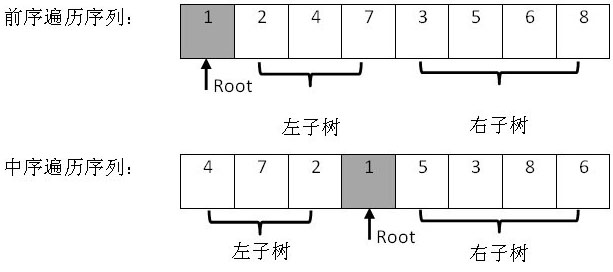
\includegraphics[scale = 0.7]{preOrderTree.jpg}
				\end{figure}
				
				分别找到了左、右子树的前序遍历序列和中序遍历序列,我们就可以用同样的方法分别去构建左右子树。换句话说,这是一个递归的过程。
			
			\subparagraph{思路总结}:先根据前序遍历序列的第一个数字创建根结点,接下来在中序遍历序列中找到根结点的位置,这样就能确定左、右子树结点的数量。在前序遍历和中序遍历的序列中划分了左、右子树结点的值之后,就可以递归地去分别构建它的左右子树。
			
			\subparagraph{要点}
				\begin{itemize}[itemindent = 1em]
					\item 边界条件 \verb|preOrder 与 inOrder| 是否为空
					\item 终止条件 \verb|leftLength > 0 与 rightLength > 0|时才重构子树
					\item 分解子树
				\end{itemize}
			\begin{lstlisting}
	public static Node<int> Construct(int[] preOrder, int[] inOrder, int length)
	{
		// 空指针判断
		if (preOrder == null || inOrder == null || length <= 0)
		{
			return null;
		}
		
		return ConstructCore(preOrder, 0, preOrder.Length - 1, inOrder, 0, inOrder.Length - 1);
	}
	
	public static Node<int> ConstructCore(int[] preOrder, int startPreOrder, int endPreOrder, int[] inOrder, int startInOrder, int endInOrder)
	{
		// 前序遍历序列的第一个数字是根结点的值
		int rootValue = preOrder[startPreOrder];
		Node<int> root = new Node<int>();
		root.data = rootValue;
		root.lchild = root.rchild = null;
		
		if (startPreOrder == endPreOrder)
		{
			if (startInOrder == endInOrder && 
			preOrder[startPreOrder] == inOrder[startInOrder])
			{
				return root;
			}
			else
			{
				throw new Exception("Invalid input!");
			}
		}
		
		// 在中序遍历中找到根结点的值
		int rootInOrder = startInOrder;
		while (rootInOrder <= endInOrder && inOrder[rootInOrder] != rootValue)
		{
			rootInOrder++;
		}
		
		// 输入的两个序列不匹配的情况
		if (rootInOrder == endInOrder && inOrder[rootInOrder] != rootValue)
		{
			throw new Exception("Invalid input!");
		}
		
		int leftLength = rootInOrder - startInOrder;
		int leftPreOrderEnd = startPreOrder + leftLength;
		if (leftLength > 0)
		{
				// 构建左子树
				root.lchild = ConstructCore(preOrder, startPreOrder + 1, leftPreOrderEnd, inOrder, startInOrder, rootInOrder - 1);
		}
		if (leftLength < endPreOrder - startPreOrder)
		{
				// 构建右子树
				root.rchild = ConstructCore(preOrder, leftPreOrderEnd + 1, endPreOrder, inOrder, rootInOrder + 1, endInOrder);
		}
		
		return root;
	}
			\end{lstlisting}
		
		\subsection{分层遍历二叉树}
			\begin{itemize}
				\item 递归
				\item 如何体现层次化
			\end{itemize}
			
			\begin{lstlisting}
	void printLevelNode_index(Node* pRoot)  
	{  
		int iCur = 0,iLast = 1;//初始化游标起始位置和当前层结束位置的下一个位置  
		vector<Node*> vecNode;  
		vecNode.push_back(pRoot);  
		while(iCur < vecNode.size())//这里应该是层结束位置等于数组大小的时候结束循环  
		{  
			iLast = vecNode.size();//牛逼,直接用当前层结束位置的下一位置 等于 向量大小 来解决了每次的更新层结束位置的问题  
			while(iCur < iLast)  
			{  
				Node* pNode = vecNode[iCur];  
				printf("%d ",pNode->_iVal);//应该先打印出当前节点值  
				if(pNode->_pLeft)  
				{  
					vecNode.push_back(pNode->_pLeft);  
				}  
				if(pNode->_pRight)  
				{  
					vecNode.push_back(pNode->_pRight);  
				}  
				iCur++;  
			}  
			printf("\n");  
		}  
	}  
			\end{lstlisting}
			
		\subsection{二分查找}
			\subsubsection{核心}
				\begin{itemize}
					\item  防止溢出 \verb| mid =  minIndex + (maxIndex - minIndex)/2 |
					\item  结束条件 \verb| while( left <= right )|
				\end{itemize}
	
	\section{数学游戏}
		\subsection{金刚坐飞机问题}
		
		\subsection{瓷砖覆盖地板}
		
		\subsection{买票找零}
		
		\subsection{点是否在三角形内}
		
		\subsection{磁带文件存放优化}
		
		\subsection{桶中取黑白球}
		
		\subsection{蚂蚁爬杆}
		
		\subsection{三角形测试用例}
		
		\subsection{数独知多少}
		
		\subsection{数字哑谜和回文}
		
		\subsection{扫雷游戏的概率}
	
	
\chapter{Array- 80}
	\section{Two Sum} 
	\subsection{问题}
		Given an array of integers, return \textbf{indices} of the two numbers such that they add up to a specific target.	
		You may assume that each input would have exactly one solution.	
		
		\subparagraph{Example}
		Given nums = [2, 7, 11, 15], target = 9,
		
		Because nums[0] + nums[1] = 2 + 7 = 9,
		
		return [0, 1].
	\subsection{解答}
	\subsection{Normal-两层循环}
	\subsection{Good-HashTable:HashMap}
	\begin{itemize}
		\item \textbf{Time complexity} : O(n). We traverse the list containing n elements only once. Each look up in the table costs only O(1) time.
		
		\item \textbf{Space complexity} :O(n).The extra space required depends on the number of items stored in the hash table, which stores at most n elements.
	\end{itemize}
	\begin{lstlisting}
	//\\\\\\\\\\\\\\\\\\\\\\\\\\Two-pass Hash Table\\\\\\\\\\\\\\\\\\\\\\\\\\\
	#include <unordered_map>
	class Solution {
	public:
		vector<int> twoSum(vector<int>& nums, int target) {
		vector<int> result;
		unordered_multimap<int, int> intergers;
		for(int i = 0; i < nums.size(); ++i)
		{
			// map 的插入值操作
			intergers.insert(pair<int,int>(nums[i],i));
		}
		
		for(unordered_multimap<int, int>::const_iterator d = intergers.begin(); d != intergers.end(); ++d)
		{
			unordered_multimap<int, int>::const_iterator find_it = intergers.find(target - d->first);
			if(find_it != intergers.end() && find_it -> second != d -> second)
			{
				result.push_back(d->second);
				result.push_back(find_it -> second);
				break;
			}
		}
		// sort 函数使用
		sort(result.begin(),result.end());
		return result;
		}		
	};
	
	//\\\\\\\\\\\\\\\\\\\\\\\\\\One-Pass HashTable\\\\\\\\\\\\\\\\\\\\\\\\\\\\\\
	Java:
	public int[] twoSum(int[] nums, int target) {
		Map<Integer, Integer> map = new HashMap<>();
		for (int i = 0; i < nums.length; i++) {
			int complement = target - nums[i];
			if (map.containsKey(complement)) {
				return new int[] { map.get(complement), i };
			}
			map.put(nums[i], i);
		}
		throw new IllegalArgumentException("No two sum solution");
	}
	\end{lstlisting}
\section{Median of Two Sorted Arrays}
		There are two sorted arrays nums1 and nums2 of size m and n respectively.
		
		Find the median of the two sorted arrays. The overall run time complexity should be O(log (m+n)).
	\subparagraph{Examples}
		nums1 = [1, 3]
		nums2 = [2]
		
		The median is 2.0
		
		nums1 = [1, 2]
		nums2 = [3, 4]
		
		The median is (2 + 3)/2 = 2.5
	\subsection{分析}
	
	\subsection{解答}
	
\section{Word Ladder II}
		Given two words (beginWord and endWord), and a dictionary's word list, find all shortest transformation sequence(s) from beginWord to endWord, such that:
		
		1-Only one letter can be changed at a time
		
		2-Each transformed word must exist in the word list. Note that beginWord is not a transformed word.
		
		Note:
		
		Return an empty list if there is no such transformation sequence.\\
		All words have the same length.\\
		All words contain only lowercase alphabetic characters.\\
		You may assume no duplicates in the word list.\\
		You may assume beginWord and endWord are non-empty and are not the same.
	\subparagraph{Examples}
		Given:
		
		beginWord = "hit"
		
		endWord = "cog"
		
		wordList = ["hot","dot","dog","lot","log","cog"]
		
		Return
		
		[
		
	\	["hit","hot","dot","dog","cog"],
		
	\	["hit","hot","lot","log","cog"]
		
		]
	\subsection{分析}
	
	\subsection{解答}
		\url{http://www.cnblogs.com/ShaneZhang/p/3748494.html}
	
\section{4Sum}
	Given an array S of n integers, are there elements a, b, c, and d in S such that a + b + c + d = target? Find all unique quadruplets in the array which gives the sum of target.
	
	Note: The solution set must not contain duplicate quadruplets.
	\subparagraph{Examples}
		given array S = [1, 0, -1, 0, -2, 2], and target = 0.
		
		A solution set is:
		
		[
		
		[-1,  0, 0, 1],
		
		[-2, -1, 1, 2],
		
		[-2,  0, 0, 2]
		
		]
	\subsection{分析}
	
	\subsection{解答}
	
	
\section{Rotate Array}
		Rotate an array of n elements to the right by k steps.
		
		Note:
		Try to come up as many solutions as you can, there are at least 3 different ways to solve this problem.
	\subparagraph{Examples}
		with n = 7 and k = 3, the array [1,2,3,4,5,6,7] is rotated to [5,6,7,1,2,3,4].
	\subsection{分析}
	
	\subsection{解答}
	
	
	
\section{Maximum Product Subarray}
		Find the contiguous subarray within an array (containing at least one number) which has the largest product.
		
	\subparagraph{Examples}
			Given the array [2,3,-2,4],
			
			the contiguous subarray [2,3] has the largest product = 6.
	\subsection{分析}
	
	\subsection{解答}
	
	
\section{Spiral Matrix}
		Given a matrix of m x n elements (m rows, n columns), return all elements of the matrix in spiral order.
	\subparagraph{Examples}
		Given the following matrix:
		
		[
		
		[ 1, 2, 3 ],
		
		[ 4, 5, 6 ],
		
		[ 7, 8, 9 ]
		
		]
		
		You should return [1,2,3,6,9,8,7,4,5].
	\subsection{分析}
	
	\subsection{解答}
	
	
\section{First Missing Positive}
		Given an unsorted integer array, find the first missing positive integer.
	\subparagraph{Examples}
		Given [1,2,0] return 3,
		
		and [3,4,-1,1] return 2.
		
		Your algorithm should run in O(n) time and uses constant space.
	\subsection{分析}
	
	\subsection{解答}
	
	
\section{Word Search}
		Given a 2D board and a word, find if the word exists in the grid.
		
		The word can be constructed from letters of sequentially adjacent cell, where "adjacent" cells are those horizontally or vertically neighboring. The same letter cell may not be used more than once.
	\subparagraph{Examples}
		Given board =
		
		[
		
		['A','B','C','E'],
		
		['S','F','C','S'],
		
		['A','D','E','E']
		
		]
		
		word = "ABCCED", -> returns true,
		
		word = "SEE", -> returns true,
		
		word = "ABCB", -> returns false.
	\subsection{分析}
	
	\subsection{解答}
	
	
\section{Largest Rectangle in Histogram}
		Given n non-negative integers representing the histogram's bar height where the width of each bar is 1, find the area of largest rectangle in the histogram.
			
	\subparagraph{Examples}
		\begin{figure}[h]
			\centering
			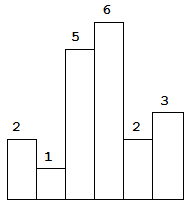
\includegraphics[scale = 0.7]{LargestH_1.png}
			\caption{Above is a histogram where width of each bar is 1, given height = [2,1,5,6,2,3]}
		\end{figure}
		\begin{figure}[h]
			\centering
			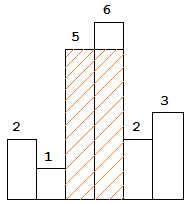
\includegraphics[scale = 0.7]{LargestH_2.png}
			\caption{The largest rectangle is shown in the shaded area, which has area = 10 unit.}
		\end{figure}
		
		Given heights = [2,1,5,6,2,3],
		
		return 10.
	\subsection{分析}
	
	\subsection{解答}
	
	
\section{Jump Game II}
		Given an array of non-negative integers, you are initially positioned at the first index of the array.
		
		Each element in the array represents your maximum jump length at that position.
		
		Your goal is to reach the last index in the minimum number of jumps.
	\subparagraph{Examples}
		Given array A = [2,3,1,1,4]
		
		The minimum number of jumps to reach the last index is 2. (Jump 1 step from index 0 to 1, then 3 steps to the last index.)
		
		Note:
		You can assume that you can always reach the last index.
	\subsection{分析}
	
	\subsection{解答}
	
	
\section{Maximal Rectangle}
		Given a 2D binary matrix filled with 0's and 1's, find the largest rectangle containing only 1's and return its area.
	\subparagraph{Examples}
		given the following matrix:
		
		1 0 1 0 0
		
		1 0 1 1 1
		
		1 1 1 1 1
		
		1 0 0 1 0
		
		Return 6.
	\subsection{分析}
	
	\subsection{解答}
	
\chapter{Hash Table- 52}
\section{Longest Substring Without Repeating Characters}
	\subsubsection{问题}
	Given a string, find the length of the longest substring without repeating characters.
	
	\subparagraph{Examples}		
	Given "abcabcbb", the answer is "abc", which the length is 3.
	
	Given "bbbbb", the answer is "b", with the length of 1.
	
	Given "pwwkew", the answer is "wke", with the length of 3. Note that the answer must be a substring, "pwke" is a subsequence and not a substring.
	
	\subsubsection{分析}
	如果发现重复:第一个指针 指向以查找的序列的最后一个该字符, 另一个指向当前的,求取最长的中间长度。
	\subsubsection{解答}
	\begin{lstlisting}
	class Solution {
	public:
	int lengthOfLongestSubstring(string s) 
	{
		int maxLen = 0,repeatCharacter_First_index = -1;
		unordered_multimap<char,int> subString;
		for (int i = 0; i < s.length(); ++i)
		{
			unordered_multimap<char,int>::const_iterator it = subString.find(s[i]);
			if (it != subString.end())
			{
				int max_second = it->second;
				auto range = subString.equal_range(s[i]);
				for_each(range.first,range.second,[&max_second](unordered_multimap<char, int>::value_type& x){max_second = max(max_second, x.second); });
				repeatCharacter_First_index = max(repeatCharacter_First_index, max_second);	// [...First_max]...Second_not insert
			}
			subString.insert(pair<char, int>(s[i], i));
			maxLen = max(maxLen, i - repeatCharacter_First_index );
		}
		return maxLen;
	}
	};
	\end{lstlisting}
	
\section{}
	
	\subparagraph{Examples}
	
	\subsection{分析}
	
	\subsection{解答}
	
\section{}
	
	\subparagraph{Examples}
	
	\subsection{分析}
	
	\subsection{解答}
	
\section{}
	
	\subparagraph{Examples}
	
	\subsection{分析}
	
	\subsection{解答}
	
	
\section{}
	
	\subparagraph{Examples}
	
	\subsection{分析}
	
	\subsection{解答}
	
	
\section{}
	
	\subparagraph{Examples}
	
	\subsection{分析}
	
	\subsection{解答}
	
	
\section{}
	
	\subparagraph{Examples}
	
	\subsection{分析}
	
	\subsection{解答}
	
	
\section{}
	
	\subparagraph{Examples}
	
	\subsection{分析}
	
	\subsection{解答}
	
	
\section{}
	
	\subparagraph{Examples}
	
	\subsection{分析}
	
	\subsection{解答}
\chapter{Linked List- 27}
	\url{http://blog.csdn.net/luckyxiaoqiang/article/details/7393134/}
\section{将单链表反转}
	
	\subsection{解答}
	
	
\section{查找单链表中的倒数第K个结点(k > 0)}
		双指针
	\subsection{解答}
	
	
\section{查找单链表的中间结点}
		双指针
	\subsection{解答}
	
	
\section{从尾到头打印单链表}
	
	\subparagraph{Examples}
	
	\subsection{分析}
	
	\subsection{解答}
	
	
\section{已知两个单链表pHead1 和pHead2 各自有序,把它们合并成一个链表依然有序}
	
	\subparagraph{Examples}
	
	\subsection{分析}
	
	\subsection{解答}
	
	
\section{判断一个单链表中是否有环}
	
	\subparagraph{Examples}
	
	\subsection{分析}
	
	\subsection{解答}
	
	
\section{判断两个单链表是否相交}
	
	\subsection{分析}
		\url{http://blog.csdn.net/jiqiren007/article/details/6572685}
		
		方法1.将第一个链表的尾部指向第二个链表,如果相交则必产生环,且环的头结点为第二个链表的头结点,没有相交则不存在环。 
		
		方法2.如果两个链表相交,则相交后的节点都一样,所以结尾节点也将一样,我们以此遍历第一个第二个链表,取出其尾部地址,判断是否相等即可。
	\subsection{解答}
	
	
\section{求两个单链表相交的第一个节点}
	
	\subparagraph{Examples}
	
	\subsection{分析}
	
	\subsection{解答}
	
	
\section{已知一个单链表中存在环,求进入环中的第一个节点}
	
	\subparagraph{Examples}
	
	\subsection{分析}
	
	\subsection{解答}
	

\section{给出一单链表头指针pHead和一节点指针pToBeDeleted,O(1)时间复杂度删除节点pToBeDeleted}
	\subsection{分析}
		对于删除节点,我们普通的思路就是让该节点的前一个节点指向该节点的下一个节点,这种情况需要遍历找到该节点的前一个节点,\textbf{时间复杂度为O(n)}。对于链表,\textbf{链表中的每个节点结构都是一样的,所以我们可以把该节点的下一个节点的数据复制到该节点,然后删除下一个节点即可}。要注意最后一个节点的情况,这个时候只能用常见的方法来操作,先找到前一个节点,但总体的平均时间复杂度还是O(1)。
	\subsection{解答}

\chapter{Math- 58}
\section{}
	
	\subparagraph{Examples}
	
	\subsection{分析}
	
	\subsection{解答}
	
\section{}
	
	\subparagraph{Examples}
	
	\subsection{分析}
	
	\subsection{解答}
	
\section{}
	\subparagraph{Examples}
	
	\subsection{分析}
	
	\subsection{解答}
	
\section{}
	
	\subparagraph{Examples}
	
	\subsection{分析}
	
	\subsection{解答}
	
\section{}
	
	\subparagraph{Examples}
	
	\subsection{分析}
	
	\subsection{解答}
	
\section{}
	
	\subparagraph{Examples}
	
	\subsection{分析}
	
	\subsection{解答}
	
\section{}
	
	\subparagraph{Examples}
	
	\subsection{分析}
	
	\subsection{解答}
	
\section{}
	
	\subparagraph{Examples}
	
	\subsection{分析}
	
	\subsection{解答}
	
\section{}
	
	\subparagraph{Examples}
	
	\subsection{分析}
	
	\subsection{解答}
	
\section{}
	
	\subparagraph{Examples}
	
	\subsection{分析}
	
	\subsection{解答}
\chapter{Two Pointers- 33}
\section{}
	
	\subparagraph{Examples}
	
	\subsection{分析}
	
	\subsection{解答}
	
\section{}
	
	\subparagraph{Examples}
	
	\subsection{分析}
	
	\subsection{解答}

\section{}	
	\subparagraph{Examples}
	
	\subsection{分析}
	
	\subsection{解答}
	
\section{}
	
	\subparagraph{Examples}
	
	\subsection{分析}
	
	\subsection{解答}
	
\section{}
	
	\subparagraph{Examples}
	
	\subsection{分析}
	
	\subsection{解答}
	
\section{}
	
	\subparagraph{Examples}
	
	\subsection{分析}
	
	\subsection{解答}
	
\section{}
	
	\subparagraph{Examples}
	
	\subsection{分析}
	
	\subsection{解答}
	
\section{}
	
	\subparagraph{Examples}
	
	\subsection{分析}
	
	\subsection{解答}
	
\section{}
	
	\subparagraph{Examples}
	
	\subsection{分析}
	
	\subsection{解答}
	
\section{}
	
	\subparagraph{Examples}
	
	\subsection{分析}
	
	\subsection{解答}
\chapter{String- 55}
	
\section{}
	
	\subparagraph{Examples}
	
	\subsection{分析}
	
	\subsection{解答}
	
\section{}
	
	\subparagraph{Examples}
	
	\subsection{分析}
	
	\subsection{解答}
	
	
\section{}
	
	\subparagraph{Examples}
	
	\subsection{分析}
	
	\subsection{解答}
	
	
\section{}
	
	\subparagraph{Examples}
	
	\subsection{分析}
	
	\subsection{解答}
	
\section{}
	
	\subparagraph{Examples}
	
	\subsection{分析}
	
	\subsection{解答}
	
	
\section{}
	
	\subparagraph{Examples}
	
	\subsection{分析}
	
	\subsection{解答}
	
	
\section{}
	
	\subparagraph{Examples}
	
	\subsection{分析}
	
	\subsection{解答}
	
	
\section{}
	
	\subparagraph{Examples}
	
	\subsection{分析}
	
	\subsection{解答}
	
\section{}
	
	\subparagraph{Examples}
	
	\subsection{分析}
	
	\subsection{解答}
	
\section{}
	
	\subparagraph{Examples}
	
	\subsection{分析}
	
	\subsection{解答}
	
\section{}
	
	\subparagraph{Examples}
	
	\subsection{分析}
	
	\subsection{解答}
	
	
\section{}
	
	\subparagraph{Examples}
	
	\subsection{分析}
	
	\subsection{解答}
	
	
\section{}
	
	\subparagraph{Examples}
	
	\subsection{分析}
	
	\subsection{解答}
	
\section{}
	
	\subparagraph{Examples}
	
	\subsection{分析}
	
	\subsection{解答}
	
\section{}
	
	\subparagraph{Examples}
	
	\subsection{分析}
	
	\subsection{解答}
\section{Divide and Conquer- 12}
\section{}
	
	\subparagraph{Examples}
	
	\subsection{分析}
	
	\subsection{解答}
	
\section{}
	
	\subparagraph{Examples}
	
	\subsection{分析}
	
	\subsection{解答}
	
	
\section{}
	
	\subparagraph{Examples}
	
	\subsection{分析}
	
	\subsection{解答}
	
\section{}
	
	\subparagraph{Examples}
	
	\subsection{分析}
	
	\subsection{解答}
	
\section{}
	
	\subparagraph{Examples}
	
	\subsection{分析}
	
	\subsection{解答}
	
\section{}
	
	\subparagraph{Examples}
	
	\subsection{分析}
	
	\subsection{解答}
	
\section{}
	
	\subparagraph{Examples}
	
	\subsection{分析}
	
	\subsection{解答}
	
\section{}
	
	\subparagraph{Examples}
	
	\subsection{分析}
	
	\subsection{解答}
	
\section{}
	
	\subparagraph{Examples}
	
	\subsection{分析}
	
	\subsection{解答}
	
\section{}
	
	\subparagraph{Examples}
	
	\subsection{分析}
	
	\subsection{解答}
\chapter{Binary Search- 38}

\section{}
	
	\subparagraph{Examples}
	
	\subsection{分析}
	
	\subsection{解答}
	
\section{}
	
	\subparagraph{Examples}
	
	\subsection{分析}
	
	\subsection{解答}
	
\section{}
	
	\subparagraph{Examples}
	
	\subsection{分析}
	
	\subsection{解答}
	
\section{}
	
	\subparagraph{Examples}
	
	\subsection{分析}
	
	\subsection{解答}
	
\section{}
	
	\subparagraph{Examples}
	
	\subsection{分析}
	
	\subsection{解答}
	
\section{}
	
	\subparagraph{Examples}
	
	\subsection{分析}
	
	\subsection{解答}
	
\section{}
	
	\subparagraph{Examples}
	
	\subsection{分析}
	
	\subsection{解答}
	
\section{}
	
	\subparagraph{Examples}
	
	\subsection{分析}
	
	\subsection{解答}
	
\section{}
	
	\subparagraph{Examples}
	
	\subsection{分析}
	
	\subsection{解答}
	
\section{}
	
	\subparagraph{Examples}
	
	\subsection{分析}
	
	\subsection{解答}
\chapter{Dynamic Programming- 66}
\section{}
	
	\subparagraph{Examples}
	
	\subsection{分析}
	
	\subsection{解答}
	
\section{}
	
	\subparagraph{Examples}
	
	\subsection{分析}
	
	\subsection{解答}
	
\section{}
	
	\subparagraph{Examples}
	
	\subsection{分析}
	
	\subsection{解答}
	
\section{}
	
	\subparagraph{Examples}
	
	\subsection{分析}
	
	\subsection{解答}
	
\section{}
	
	\subparagraph{Examples}
	
	\subsection{分析}
	
	\subsection{解答}
	
\section{}
	
	\subparagraph{Examples}
	
	\subsection{分析}
	
	\subsection{解答}
	
\section{}
	
	\subparagraph{Examples}
	
	\subsection{分析}
	
	\subsection{解答}
	
\section{}
	
	\subparagraph{Examples}
	
	\subsection{分析}
	
	\subsection{解答}
	
	
\section{}
	
	\subparagraph{Examples}
	
	\subsection{分析}
	
	\subsection{解答}
	
	
\section{}
	
	\subparagraph{Examples}
	
	\subsection{分析}
	
	\subsection{解答}
	
\section{}
	
	\subparagraph{Examples}
	
	\subsection{分析}
	
	\subsection{解答}
	
\section{}
	
	\subparagraph{Examples}
	
	\subsection{分析}
	
	\subsection{解答}
	
\section{}
	
	\subparagraph{Examples}
	
	\subsection{分析}
	
	\subsection{解答}
	
\section{}
	
	\subparagraph{Examples}
	
	\subsection{分析}
	
	\subsection{解答}
	
\section{}
	
	\subparagraph{Examples}
	
	\subsection{分析}
	
	\subsection{解答}
	
\section{}
	
	\subparagraph{Examples}
	
	\subsection{分析}
	
	\subsection{解答}
	
\section{}
	
	\subparagraph{Examples}
	
	\subsection{分析}
	
	\subsection{解答}
	
\section{}
	
	\subparagraph{Examples}
	
	\subsection{分析}
	
	\subsection{解答}
\chapter{Backtracking- 34}
\section{}
	
	\subparagraph{Examples}
	
	\subsection{分析}
	
	\subsection{解答}
	
\section{}
	
	\subparagraph{Examples}
	
	\subsection{分析}
	
	\subsection{解答}
	
\section{}
	
	\subparagraph{Examples}
	
	\subsection{分析}
	
	\subsection{解答}
	
\section{}
	
	\subparagraph{Examples}
	
	\subsection{分析}
	
	\subsection{解答}
	
\section{}
	
	\subparagraph{Examples}
	
	\subsection{分析}
	
	\subsection{解答}
	
\section{}
	
	\subparagraph{Examples}
	
	\subsection{分析}
	
	\subsection{解答}
	
\section{}
	
	\subparagraph{Examples}
	
	\subsection{分析}
	
	\subsection{解答}
	
\chapter{Stack- 25}
\section{}
	
	\subparagraph{Examples}
	
	\subsection{分析}
	
	\subsection{解答}
	
\section{}
	
	\subparagraph{Examples}
	
	\subsection{分析}
	
	\subsection{解答}
	
\section{}
	
	\subparagraph{Examples}
	
	\subsection{分析}
	
	\subsection{解答}
	
\section{}
	
	\subparagraph{Examples}
	
	\subsection{分析}
	
	\subsection{解答}
	
\section{}
	
	\subparagraph{Examples}
	
	\subsection{分析}
	
	\subsection{解答}
\chapter{Heap- 15}
\section{}
	
	\subparagraph{Examples}
	
	\subsection{分析}
	
	\subsection{解答}
	
\section{}
	
	\subparagraph{Examples}
	
	\subsection{分析}
	
	\subsection{解答}
	
\section{}
	
	\subparagraph{Examples}
	
	\subsection{分析}
	
	\subsection{解答}
	
\section{}
	
	\subparagraph{Examples}
	
	\subsection{分析}
	
	\subsection{解答}
	
\section{}
	
	\subparagraph{Examples}
	
	\subsection{分析}
	
	\subsection{解答}
	
\section{}
	
	\subparagraph{Examples}
	
	\subsection{分析}
	
	\subsection{解答}
	
\section{}
	
	\subparagraph{Examples}
	
	\subsection{分析}
	
	\subsection{解答}
	
\section{}
	
	\subparagraph{Examples}
	
	\subsection{分析}
	
	\subsection{解答}
	
\section{}
	
	\subparagraph{Examples}
	
	\subsection{分析}
	
	\subsection{解答}
	
\section{}
	
	\subparagraph{Examples}
	
	\subsection{分析}
	
	\subsection{解答}
\chapter{Greedy- 19}
\section{}
	
	\subparagraph{Examples}
	
	\subsection{分析}
	
	\subsection{解答}
	
\section{}
	
	\subparagraph{Examples}
	
	\subsection{分析}
	
	\subsection{解答}
	
\section{}
	
	\subparagraph{Examples}
	
	\subsection{分析}
	
	\subsection{解答}
	
\section{}
	
	\subparagraph{Examples}
	
	\subsection{分析}
	
	\subsection{解答}
	
\section{}
	
	\subparagraph{Examples}
	
	\subsection{分析}
	
	\subsection{解答}
	
\section{}
	
	\subparagraph{Examples}
	
	\subsection{分析}
	
	\subsection{解答}
	
\section{}
	
	\subparagraph{Examples}
	
	\subsection{分析}
	
	\subsection{解答}
	
\section{}
	
	\subparagraph{Examples}
	
	\subsection{分析}
	
	\subsection{解答}
	
\section{}
	
	\subparagraph{Examples}
	
	\subsection{分析}
	
	\subsection{解答}
	
\section{}
	
	\subparagraph{Examples}
	
	\subsection{分析}
	
	\subsection{解答}
\chapter{Sort- 16}
\section{冒泡}
	冒泡排序的基本思想是,对\textbf{相邻的元素}进行\textbf{两两比较},顺序相反则进行交换,这样,\textbf{每一趟}会\textbf{将最小或最大的元素“浮”到顶端},最终达到完全有序
	
		\begin{figure}[h]
			\centering
			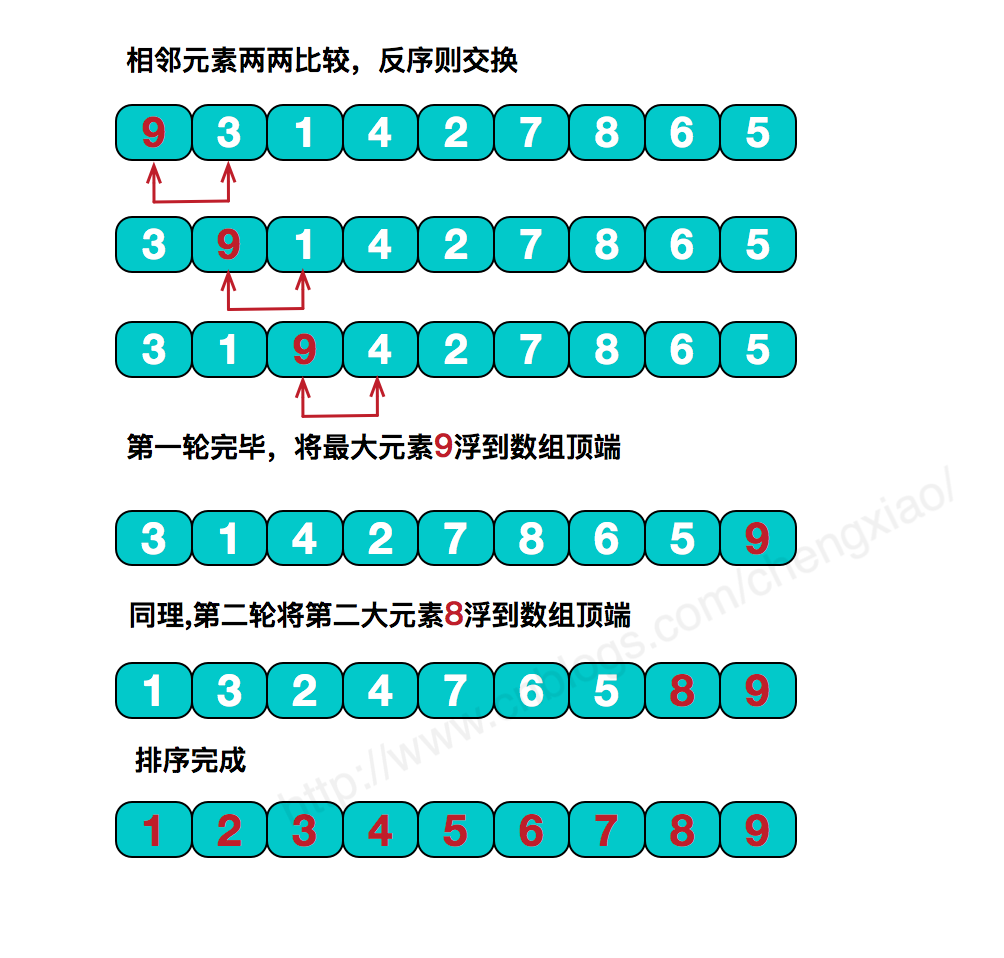
\includegraphics[scale = 0.7]{Pop.png}
		\end{figure}
	
	\subsection{解答}
	\url{https://github.com/ctzhenghua/C-NetworkPractice-Code/blob/master/DataStructure/Sort/PopSort.cc}
		
\section{选择排序}
	
	选择排序的思想非常直接,不是要排序么?那好,我就从所有序列中\textbf{先找到最小的},\textbf{然后放到第一个位置}。\textbf{之后再看剩余元素中最小的,放到第二个位置}……以此类推,就可以完成整个的排序工作了。可以很清楚的发现,选择排序是固定位置,找元素。相比于插入排序的固定元素找位置,是两种思维方式。不过条条大路通罗马,两者的目的是一样的。
	
	\subsection{解答}
	\url{https://github.com/ctzhenghua/C-NetworkPractice-Code/blob/master/DataStructure/Sort/SelectSort.cc}
		
\section{快速排序}

	快速排序是\textbf{找出一个元素}(理论上可以随便找一个)\textbf{作为基准(pivot)},然后对数组进行分区操作,\textbf{使基准左边元素的值都不大于基准值,基准右边的元素值 都不小于基准值},如此作为基准的元素调整到排序后的正确位置。递归快速排序,将其他n-1个元素也调整到排序后的正确位置。最后每个元素都是在排序后的正 确位置,排序完成。所以快速排序算法的核心算法是分区操作,即如何调整基准的位置以及调整返回基准的最终位置以便分治递归。
	
	\subsection{解答}
		\url{https://github.com/ctzhenghua/C-NetworkPractice-Code/blob/master/DataStructure/Sort/QuickSort.cc}
\section{插入排序}
	
	插入即表示将一个新的数据插入到一个有序数组中,并继续保持有序。例如有一个长度为N的无序数组,进行N-1次的插入即能完成排序;第一次,数组第1个数认为是有序的数组,将数组第二个元素插入仅有1个有序的数组中;第二次,数组前两个元素组成有序的数组,将数组第三个元素插入由两个元素构成的有序数组中......第N-1次,数组前N-1个元素组成有序的数组,将数组的第N个元素插入由N-1个元素构成的有序数组中,则完成了整个插入排序。
	
	\subsection{解答}
	
\section{归并}
	
	\url{http://www.cnblogs.com/jingmoxukong/p/4308823.html}
	
	\subsection{解答}
	
\section{堆}
	\url{http://www.cnblogs.com/mengdd/archive/2012/11/30/2796845.html}
	
		\begin{itemize}
			\item  数组最后 总是不需要再调整的
			\item  调整好后,根与当前剩下未确定的最后一个进行位置交换
		\end{itemize}
	
		\begin{figure}[h]
			\centering
			\includegraphics*[scale = 0.7]{Heap.png}
		\end{figure}
	\subsection{解答}
	
	\url{http://blog.csdn.net/xiaoxiaoxuewen/article/details/7570621/}
	
\section{}
	
	\subparagraph{Examples}
	
	\subsection{分析}
	
	\subsection{解答}
	
\section{}
	
	\subparagraph{Examples}
	
	\subsection{分析}
	
	\subsection{解答}
	
	
\section{}
	
	\subparagraph{Examples}
	
	\subsection{分析}
	
	\subsection{解答}
	
\section{}
	
	\subparagraph{Examples}
	
	\subsection{分析}
	
	\subsection{解答}
\chapter{Bit Manipulation- 26}
\section{}
	
	\subparagraph{Examples}
	
	\subsection{分析}
	
	\subsection{解答}
	
\section{}
	
	\subparagraph{Examples}
	
	\subsection{分析}
	
	\subsection{解答}
	
\section{}
	
	\subparagraph{Examples}
	
	\subsection{分析}
	
	\subsection{解答}
	
\section{}
	
	\subparagraph{Examples}
	
	\subsection{分析}
	
	\subsection{解答}
	
\section{}
	
	\subparagraph{Examples}
	
	\subsection{分析}
	
	\subsection{解答}
	
\section{}
	
	\subparagraph{Examples}
	
	\subsection{分析}
	
	\subsection{解答}
	
\section{}
	
	\subparagraph{Examples}
	
	\subsection{分析}
	
	\subsection{解答}
	
\section{}
	
	\subparagraph{Examples}
	
	\subsection{分析}
	
	\subsection{解答}
	
	
\section{}
	
	\subparagraph{Examples}
	
	\subsection{分析}
	
	\subsection{解答}
	
\section{}
	
	\subparagraph{Examples}
	
	\subsection{分析}
	
	\subsection{解答}	
\chapter{Tree- 48}
	\url{http://blog.csdn.net/luckyxiaoqiang/article/details/7518888}
\section{Binary Tree Maximum Path Sum}
		Given a binary tree, find the maximum path sum.
		
		For this problem, a path is defined as any sequence of nodes from some starting node to any node in the tree along the parent-child connections. The path must contain at least one node and does not need to go through the root.
	\subparagraph{Examples}
		Given the below binary tree,
		
		\begin{figure}[h]
			\centering
			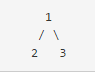
\includegraphics[scale = 1]{Tree_1.png}
		\end{figure}
		
		Return 6.	
	\subsection{分析}
	
	\subsection{解答}
		\begin{lstlisting}
	/**
	* Definition for a binary tree node.
	* struct TreeNode {
	*     int val;
	*     TreeNode *left;
	*     TreeNode *right;
	*     TreeNode(int x) : val(x), left(NULL), right(NULL) {}
	* };
	*/
	class Solution {
	public:
	int maxPathSum(TreeNode* root) {
	
	}
	};
		\end{lstlisting}
\section{Validate Binary Search Tree}
		Given a binary tree, determine if it is a valid binary search tree (BST).
		
		Assume a BST is defined as follows:
		
		1-The left subtree of a node contains only nodes with keys less than the node's key.
		
		2-The right subtree of a node contains only nodes with keys greater than the node's key.
		
		3-Both the left and right subtrees must also be binary search trees.
	\subparagraph{Examples}
		Given the below binary tree,
		
		\begin{figure}[h]
			\centering
			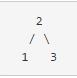
\includegraphics[scale = 1]{Tree_2.png}
		\end{figure}
		
		Binary tree [2,1,3], return true.
		
		\begin{figure}[h]
			\centering
			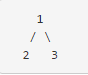
\includegraphics[scale = 1]{Tree_3.png}
		\end{figure}
		
		Binary tree [1,2,3], return false.
	\subsection{分析}
	
	\subsection{解答}
	
\section{求二叉树中的节点个数}
	\subsection{分析}
	
	\subsection{解答}
	
\section{求二叉树的深度}
	\subsection{分析}
	
	\subsection{解答}
	
\section{前序遍历,中序遍历,后序遍历}
	\subsection{分析}
	
	\subsection{解答}
	
\section{分层遍历二叉树(按层次从上往下,从左往右)}
	\subsection{分析}
	
	\subsection{解答}
	
\section{将二叉查找树变为有序的双向链表}
	\subsection{分析}
	
	\subsection{解答}
	
\section{求二叉树第K层的节点个数}
	\subsection{分析}
	
	\subsection{解答}
	
	
\section{求二叉树中叶子节点的个数}
	\subsection{分析}
	
	\subsection{解答}
	
\section{判断两棵二叉树是否结构相同}
	\subsection{分析}
	
	\subsection{解答}
\section{判断二叉树是不是平衡二叉树}
	\subsection{分析}
	
	\subsection{解答}
	
\section{求二叉树的镜像}
	\subsection{分析}
	
	\subsection{解答}
	
\section{求二叉树中两个节点的最低公共祖先节点}
	\subsection{分析}
	
	\subsection{解答}
	
\section{求二叉树中节点的最大距离}
	\subsection{分析}
	
	\subsection{解答}
	
\section{由前序遍历序列和中序遍历序列重建二叉树}
	\subsection{分析}
	
	\subsection{解答}
	
\section{判断二叉树是不是完全二叉树}
	\subsection{分析}
	
	\subsection{解答}
	
\chapter{Depth-first Search- 41}
\section{部分和问题}
	给定整数$a_1, a_2,...,a_n$,判断是否可以从中选出若干数,使他们的和恰好为$k$
	\subparagraph{Examples}
		\begin{lstlisting}[frame = ,xleftmargin=.02\textwidth]
// Test Case 1
	输入
	n = 4
	a = {1, 2, 4, 7}
	k = 13
	
	输出
	Yes{13 = 2 + 4 + 7}
// Test Case 2
	输入
	n = 4
	a = {1, 2, 4, 7}
	k = 15
	
	输出
	No
		\end{lstlisting}
	\subsection{分析}
	
	当$n < 20$时,运算次数为100 0000 次,可以接受
	\subsection{解答}
		\begin{lstlisting}
	int a[MAX_N];
	int n, k;
	
	bool dfs(int i, sum)
	{
		if(i == n) return sum == k;
		if(dfs(i+1, sum)) return true;
		if(dfs(i+1, sum+a[i])) return true;
		return false;
	}
		\end{lstlisting}
	
\section{}
	
	\subparagraph{Examples}
	
	\subsection{分析}
	
	\subsection{解答}
	
\section{}
	
	\subparagraph{Examples}
	
	\subsection{分析}
	
	\subsection{解答}
	
\section{}
	
	\subparagraph{Examples}
	
	\subsection{分析}
	
	\subsection{解答}
	
\section{}
	
	\subparagraph{Examples}
	
	\subsection{分析}
	
	\subsection{解答}
	
\section{}
	
	\subparagraph{Examples}
	
	\subsection{分析}
	
	\subsection{解答}
	
\section{}
	
	\subparagraph{Examples}
	
	\subsection{分析}
	
	\subsection{解答}
	
\section{}
	
	\subparagraph{Examples}
	
	\subsection{分析}
	
	\subsection{解答}
	
	
\section{}
	
	\subparagraph{Examples}
	
	\subsection{分析}
	
	\subsection{解答}
	
\section{}
	
	\subparagraph{Examples}
	
	\subsection{分析}
	
	\subsection{解答}
\chapter{Breadth-first Search- 21}
\section{}
	
	\subparagraph{Examples}
	
	\subsection{分析}
	
	\subsection{解答}
	
\section{}
	
	\subparagraph{Examples}
	
	\subsection{分析}
	
	\subsection{解答}
	
\section{}
	
	\subparagraph{Examples}
	
	\subsection{分析}
	
	\subsection{解答}
	
\section{}
	
	\subparagraph{Examples}
	
	\subsection{分析}
	
	\subsection{解答}
	
\section{}
	
	\subparagraph{Examples}
	
	\subsection{分析}
	
	\subsection{解答}
	
\section{}
	
	\subparagraph{Examples}
	
	\subsection{分析}
	
	\subsection{解答}
	
\section{}
	
	\subparagraph{Examples}
	
	\subsection{分析}
	
	\subsection{解答}
	
\section{}
	
	\subparagraph{Examples}
	
	\subsection{分析}
	
	\subsection{解答}
	
	
\section{}
	
	\subparagraph{Examples}
	
	\subsection{分析}
	
	\subsection{解答}
	
\section{}
	
	\subparagraph{Examples}
	
	\subsection{分析}
	
	\subsection{解答}
\chapter{Union Find- 6}	
\section{}
	
	\subparagraph{Examples}
	
	\subsection{分析}
	
	\subsection{解答}
	
\section{}
	
	\subparagraph{Examples}
	
	\subsection{分析}
	
	\subsection{解答}
	
	
\section{}
	
	\subparagraph{Examples}
	
	\subsection{分析}
	
	\subsection{解答}
	
\section{}
	
	\subparagraph{Examples}
	
	\subsection{分析}
	
	\subsection{解答}
\chapter{Graph- 10}
\section{}
	
	\subparagraph{Examples}
	
	\subsection{分析}
	
	\subsection{解答}
	
\section{}
	
	\subparagraph{Examples}
	
	\subsection{分析}
	
	\subsection{解答}
	
\section{}
	
	\subparagraph{Examples}
	
	\subsection{分析}
	
	\subsection{解答}
	
\section{}
	
	\subparagraph{Examples}
	
	\subsection{分析}
	
	\subsection{解答}
	
\section{}
	
	\subparagraph{Examples}
	
	\subsection{分析}
	
	\subsection{解答}
\section{}
	
	\subparagraph{Examples}
	
	\subsection{分析}
	
	\subsection{解答}
	
\section{}
	
	\subparagraph{Examples}
	
	\subsection{分析}
	
	\subsection{解答}
	
\section{}
	
	\subparagraph{Examples}
	
	\subsection{分析}
	
	\subsection{解答}
	
\section{}
	
	\subparagraph{Examples}
	
	\subsection{分析}
	
	\subsection{解答}
	
\section{}
	
	\subparagraph{Examples}
	
	\subsection{分析}
	
	\subsection{解答}
\chapter{Design- 27}
\section{}
	
	\subparagraph{Examples}
	
	\subsection{分析}
	
	\subsection{解答}
	
\section{}
	
	\subparagraph{Examples}
	
	\subsection{分析}
	
	\subsection{解答}
	
\section{}
	
	\subparagraph{Examples}
	
	\subsection{分析}
	
	\subsection{解答}
	
\section{}
	
	\subparagraph{Examples}
	
	\subsection{分析}
	
	\subsection{解答}
	
\section{}
	
	\subparagraph{Examples}
	
	\subsection{分析}
	
	\subsection{解答}
	
\section{}
	
	\subparagraph{Examples}
	
	\subsection{分析}
	
	\subsection{解答}
	
\section{}
	
	\subparagraph{Examples}
	
	\subsection{分析}
	
	\subsection{解答}
	
\section{}
	
	\subparagraph{Examples}
	
	\subsection{分析}
	
	\subsection{解答}
	
\section{}
	
	\subparagraph{Examples}
	
	\subsection{分析}
	
	\subsection{解答}
	
\section{}
	
	\subparagraph{Examples}
	
	\subsection{分析}
	
	\subsection{解答}
\chapter{Topological Sort[拓扑排序]- 5}
\section{}
	
	\subparagraph{Examples}
	
	\subsection{分析}
	
	\subsection{解答}
	
\section{}
	
	\subparagraph{Examples}
	
	\subsection{分析}
	
	\subsection{解答}
	
\section{}
	
	\subparagraph{Examples}
	
	\subsection{分析}
	
	\subsection{解答}
\chapter{Trie[前缀-字典树]- 7}
\section{}
	
	\subparagraph{Examples}
	
	\subsection{分析}
	
	\subsection{解答}
	
\section{}
	
	\subparagraph{Examples}
	
	\subsection{分析}
	
	\subsection{解答}
	
\section{}
	
	\subparagraph{Examples}
	
	\subsection{分析}
	
	\subsection{解答}
	
\chapter{Bianry Indexed Tree- 4}
\section{}
	
	\subparagraph{Examples}
	
	\subsection{分析}
	
	\subsection{解答}
	
\section{}
	
	\subparagraph{Examples}
	
	\subsection{分析}
	
	\subsection{解答}
	
\section{}
	
	\subparagraph{Examples}
	
	\subsection{分析}
	
	\subsection{解答}
	
\chapter{Segment Tree- 4}
\section{}
	
	\subparagraph{Examples}
	
	\subsection{分析}
	
	\subsection{解答}
	
\section{}
	
	\subparagraph{Examples}
	
	\subsection{分析}
	
	\subsection{解答}
	
\section{}
	
	\subparagraph{Examples}
	
	\subsection{分析}
	
	\subsection{解答}
\chapter{Binary Search Tree- 4}
\section{}
	
	\subparagraph{Examples}
	
	\subsection{分析}
	
	\subsection{解答}
	
\section{}
	
	\subparagraph{Examples}
	
	\subsection{分析}
	
	\subsection{解答}
	
\section{}
	
	\subparagraph{Examples}
	
	\subsection{分析}
	
	\subsection{解答}

\chapter{Other Aspects}
\section{Recursion[递归]- 2}	
	\subsection{}
	
	\subparagraph{Examples}
	
	\subsection{分析}
	
	\subsection{解答}
\section{Brainteaser[谜题]- 2}
	\subsection{}
	
	\subparagraph{Examples}
	
	\subsection{分析}
	
	\subsection{解答}
\section{Memoization[以避免递归重复计算,如Fibonacci(斐波那契)问题]- 1}
	\subsection{}
	
	\subparagraph{Examples}
	
	\subsection{分析}
	
	\subsection{解答}

\section{Queue- 3}
	\subsection{}
	
		\subparagraph{Examples}
		
		\subsubsection{分析}
	
		\subsubsection{解答}
	
	\subsection{}
	
		\subparagraph{Examples}
	
		\subsubsection{分析}
	
		\subsubsection{解答}

\section{Reservoir Sampling[随机抽样]- 2}
	\subsection{}
	
		\subparagraph{Examples}
	
		\subsubsection{分析}
	
		\subsubsection{解答}
		
\section{Minimax[极小化极大算法]- 3}
	\subsection{}
	
		\subparagraph{Examples}
		
		\subsubsection{分析}
		
		\subsubsection{解答}
	\subsection{}
		
		\subparagraph{Examples}
		
		\subsubsection{分析}
		
		\subsubsection{解答}

\section{Other Interview}
\subsection{迷宫字符串} 
	\subsubsection{问题}
	已知:一个二维的字母矩阵和一个由字母组装的单词。输出:该单词是否可以从二维字母矩阵中拼接出来,拼接规则为从矩阵的某一行的某个字母开始,持续向临近的字母扩展(向上、向下、向左或向右),直至拼接出该单词。若最终可以拼接出,则输出true;若最终不可以拼接出,则输出false
	
	\subparagraph{Example}
		Given 字母矩阵为
		
			A B C D E
			
			E F G H U
			
			A B S D F
		
		输入:ABCGH  输出 true
		
		输入:FGHDSB  输出 true
		
		输入:EFGU  输出 false
	\subsubsection{解答}
		\subsubsection{队列方法}
\begin{lstlisting}
	#include <iostream>
	#include <list>
	using namespace std;
	
	struct Roud{
		int i;	 //rows
		int j;   //columns
		int now; //testCase[now];
		list<char> roud;
	};
	
	// queue
	list<Roud> all;
	list<char> result;
	
	// arrayCharacters
	char array[3][5] = { { 'A', 'B', 'C', 'D', 'E' }, { 'E', 'F', 'G', 'H', 'U' }, { 'A', 'B', 'S', 'D', 'F' } };
	
	void createReslut(char * testCase)
	{
		for (int i = 0; i < strlen(testCase); ++i)
		{
			result.push_back(testCase[i]);
		}
	}
	void solve(char * testCase)
	{
		// Checking The First Elements
		int  i = 0;
		for (int _i = 0; _i < 3; ++_i)
		{
			for (int j = 0; j < 5; ++j)
			{
				if (array[_i][j] == testCase[0])
				{
					Roud temp;
					temp.roud.push_back(testCase[0]);
					temp.i = _i;
					temp.j = j;
					temp.now = 0;
					all.push_back(temp);
					
					if (i == 0)
						++i;
				}
			}
		}
	
		// Queue Checking Roud
		while (testCase[i] != '\0' && all.size() > 0)
		{
			Roud temp = all.front();
			Roud tempN;
			if (result == temp.roud)
				break;
			
			i = temp.now;
			++i;
			// Checking 4 direction
				// Up
				if ((temp.i - 1 >= 0) && (testCase[i] == array[temp.i - 1][temp.j]))
				{
					tempN.i = temp.i - 1;
					tempN.j = temp.j;
					tempN.now = temp.now + 1;
					tempN.roud = temp.roud;
					tempN.roud.push_back(testCase[i]);
					all.push_back(tempN);
				}
				// Down
				if ((temp.i +1  <= 2) && (testCase[i] == array[temp.i + 1][temp.j]))
				{
					tempN.i = temp.i + 1;
					tempN.j = temp.j;
					tempN.now = temp.now + 1;
					tempN.roud = temp.roud;
					tempN.roud.push_back(testCase[i]);
					all.push_back(tempN);
				}
				// Left
				if ((temp.j -1 >= 0) && (testCase[i] == array[temp.i][temp.j-1]))
				{
					tempN.i = temp.i;
					tempN.j = temp.j-1;
					tempN.now = temp.now + 1;
					tempN.roud = temp.roud;
					tempN.roud.push_back(testCase[i]);
					all.push_back(tempN);
				}
				// Right
				if ((temp.j+1 <= 4) && (testCase[i] == array[temp.i][temp.j+1]))
				{
					tempN.i = temp.i;
					tempN.j = temp.j + 1;
					tempN.now = temp.now + 1;
					tempN.roud = temp.roud;
					tempN.roud.push_back(testCase[i]);
					all.push_back(tempN);
				}
				all.pop_front();
		}
			
		if (all.size()>0)
			cout << "true" << endl;
		else
			cout << "false" << endl;
	}
	
	int main()
	{
		char test[256];
		cin >> test;
		
		createReslut(test);
		solve(test);
		
		system("PAUSE");
		return 0;
	}
\end{lstlisting}


 \end{document} 
 
 
 